\documentclass[10pt]{exam}
\usepackage[hon]{template-for-exam}
\usepackage{endnotes,graphicx}
\usepackage{tikz,graphicx,enumitem,multicol,float,my-tikz-clipart,silence,cclicenses}
\graphicspath{{./figures/}}
\WarningFilter{latex}{Label `part}
\WarningFilter{latex}{There were multiply-defined labels}

\footer{}{\thepage}{\sc \myclass}


%\def\answer#1{\footnotetext{#1}}
%\def\myquestion{\item\stepcounter{footnote}}

\def\enoteheading{}
\def\answer#1{\endnotetext{#1}}
\def\theanswers{\theendnotes}
\def\myquestion{\item\stepcounter{endnote}}

\newenvironment{myquestions}{
  \begin{multicols*}{2}\begin{enumerate}
}{
  \end{enumerate}\end{multicols*}
}
\makeatletter
\patchcmd{\enit@setresumekeys}{\def}{\gdef}{}{}
\patchcmd{\enit@setresumekeys}{\def}{\gdef}{}{}
\makeatother

\newcommand{\myheading}[1]{\uplevel{\section*{#1}}
}
\newcommand{\mysubheading}[1]{\uplevel{\subsection*{#1}}
}

%uncomment if running Pandoc
% \renewcommand{\myheading}[1]{{\section*{#1}}}
% \renewcommand{\mysubheading}[1]{\subsection*{#1}}



%%%%%%%%%%%%%%%% Dates %%%%%%%%%%%%%%%%%%%
\def\quizday{Tue, Feb 10} % also used as HW Check A Day
\def\testday{Tue, Feb 24}

\def\one{Fri, Jan 30}
\def\two{Mon, Feb 2}
\def\three{Fri, Feb 6}
\def\four{Mon, Feb 9}
\def\five{We-Th, Feb 11-12}
\def\six{Fri, Feb 13}
%%%%%%%%%%%%%%%%%%%%%%%%%%%%%%%%%%%%%%%%%



\def\mytitle{Chapter 10 Homework (Rotational Motion)}
\title{\mytitle}
\date{\today}

\def\mymaketitle{
  \begin{flushleft}
    {\LARGE \textbf \mytitle \par}
  \end{flushleft}
}

\newcommand{\bs}[2]{\textbf{#1} (\sc #2 Points)}


\newcommand{\GFig}[2]{  
  \begin{figure}[H]
    \centering
    \includegraphics[width=#2]{08_#1_Figure.jpg}
    \caption{Giancolli Figure 8-#1.}
    \label{8-#1}
  \end{figure}
}


\begin{document}
\maketitle


\begin{center}
  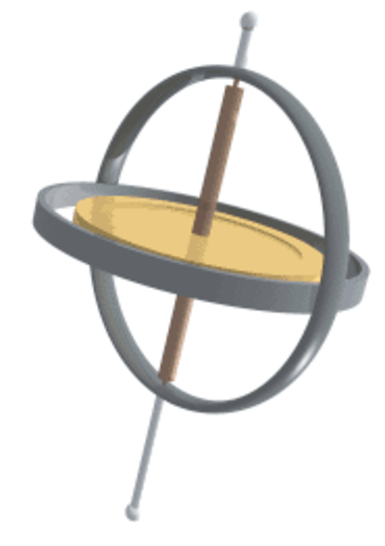
\includegraphics[height=6cm]{gyroscope.pdf}
\end{center}

\section*{HW Check A (collected on \quizday)}


%%%%%%%%%%%

\subsection*{Reading}

Please read the following on your own in the OpenStax textbook by the dates given.  It will give good context for class discussion.  Check off when you have completed them.

\vspace{1em}

\begin{checkboxes}
  \choice 6.1 (Review) Rotation Angle \& Angular Velocity \dotfill \one
  \choice 10.1 Angular Acceleration \dotfill \one
  \choice 10.2 Kinematics of Rotational Motion \dotfill \two
  \choice 9.2 The Second Condition of Equilibrium (definition of torque) \dotfill \three
\end{checkboxes}


\subsection*{Problems and Conceptual Question}


Get stamps from your instructor as you complete each of the following problems.  The conceptual questions (CQ) require at least one sentence of explanation.

\vspace{1em}

\noindent
{\sc Stamps will not be given if work is not shown on a separate sheet of paper}

\vspace{1em}


\begin{tabular}{|*{3}{p{4.8cm}|}}
  \hline
  %
  \bs{Ang. Quantities}{8}               
                    & \bs{Rot. Kin. Eqs.}{4}
                                      & \bs{Torque}{3}  \\
  Problems \#\ref{1p-i}-\ref{1p-f}
              & Problems \#\ref{2p-i}-\ref{2p-f} 
                    & Problems \#\ref{3p-i}-\ref{3p-f}\\
  Conceptual \#\ref{1q-i}-\ref{1q-f}
          & %Conceptual \#\ref{2q-i}-\ref{2q-f}
              & Conceptual \#\ref{3q-i}-\ref{3q-f} \\
          & \textbf{HW Quiz on \quizday} & \\[4em]\hline  
  %%
\end{tabular}



\pagebreak

\newcommand{\refsheet}{
  \section*{Selected Answers}

  \renewcommand{\enotesize}{\normalsize}
  \renewcommand{\enoteformat}{%
    \leftskip=1.8em
    \makebox[0pt][r]{\theenmark. }%
  }

  \hfill
  \theanswers
}

\refsheet



\pagebreak
\mymaketitle
\section*{HW Check B (collected on Test Day - \testday)}






%%%%%%%%%%%

\subsection*{Reading}

Please read the following on your own in the OpenStax textbook by the dates given.  It will give good context for class discussion.  Check off when you have completed them.

\vspace{1em}

\begin{checkboxes}
  \choice 10.3 Dynamics of Rotational Motion \dotfill \four
  \choice 10.4 Rotational Kinetic Energy \dotfill \five
  \choice 10.5 Angular Momentum \& its Conservation \dotfill \six
\end{checkboxes}


\subsection*{Problems and Conceptual Question}


Get stamps from your instructor as you complete each of the following problems.  The conceptual questions (CQ) require at least one sentence of explanation.

\vspace{1em}

\noindent
{\sc Stamps will not be given if work is not shown on a separate sheet of paper}

\vspace{1em}


\begin{tabular}{|*{3}{p{4.8cm}|}}
  \hline
  %
  \bs{Rot. Dynamics}{6}               
          & \bs{Rot. KE}{4} 
          & \bs{Ang Momentum}{5} \\
  Problems \#\ref{4p-i}-\ref{4p-f}
          & Problems \#\ref{5p-i}-\ref{5p-f} 
          & Problems \#\ref{6p-i}-\ref{6p-f}\\
  Conceptual \#\ref{4q-i}-\ref{4q-f}
          & Conceptual \#\ref{5q-i}-\ref{5q-f}
          & Conceptual \#\ref{6q-i}-\ref{6q-f} 
          \\
          & & \\[3em]\hline
  %%
\end{tabular}

\subsection*{Bonus Problems}

\hfill

\begin{tabular}{|*{3}{p{3.5cm}|}}
  \hline
  %
  \#\ref{b1}  &  \#\ref{b2}  &  \#\ref{b3}  \\[1.5cm]
  %
  \hline
\end{tabular}

\vspace{3em}

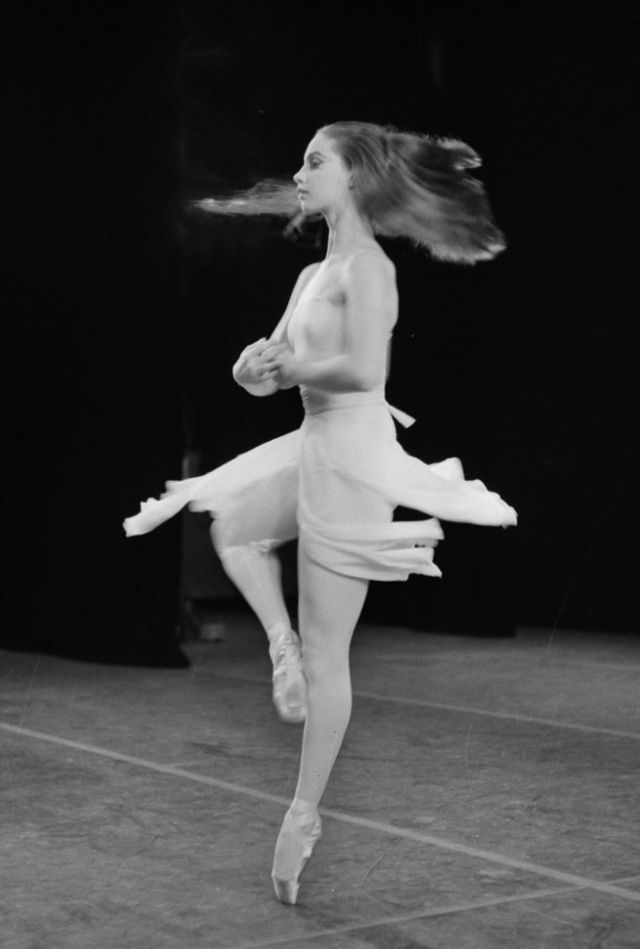
\includegraphics[height=6cm]{Suzanne_Farrell_1965.jpg} \hfill 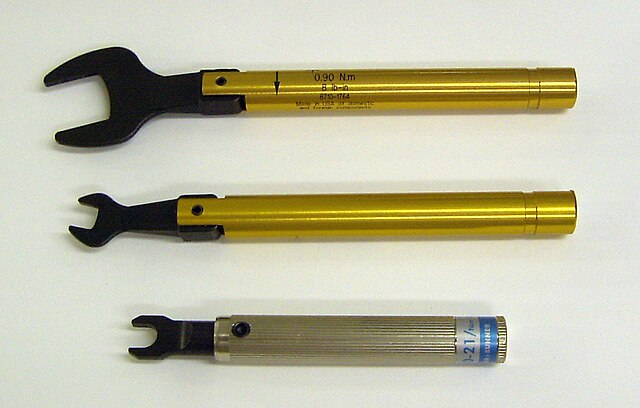
\includegraphics[height=6cm]{wrenches.JPG}

%%%%%%%%%%%%%
%%%%%%%%%%%%%


\pagebreak 
\refsheet 
\pagebreak


\noindent
Questions and figures are from OpenStax \emph{College Physics}, 2nd ed, (Chapter 10) or Giancolli \emph{Physics: Principles with Applications}, 7th ed, (Chapter 8) unless otherwise noted.
 unless otherwise noted.



\begin{myquestions}

\myheading{Angular Quantites}
\mysubheading{Problems}


\myquestion (Giancolli P1) \label{1p-i}
Express the following angles in radians: (a) $45^\circ$; (b) $60^\circ$; (c) $90^\circ$; (d) $360^\circ$; (e)~$445^\circ$.
\answer{(a) 0.79 rad; (b) 1.05 rad; (c) 1.57 rad; (d) 6.2 rad; (e) 7.77 rad}

\myquestion (P1) 
At its peak, a tornado is 60.0~m in diameter and carries 140-m/s winds. What is its angular velocity in revolutions per second?
\answer{$\SI{4.63}{rad/s}=\SI{0.737}{rev/s}$}


\myquestion (P2) \textit{Integrated Concepts.} An ultracentrifuge accelerates from rest to \SI{100000}{rpm} in 2.0~min. (a) What is its angular acceleration in \SI{}{rad/s^2}? (b) What is the tangential acceleration of a point 9.50~cm from the axis of rotation? (c) What is the radial acceleration in \SI{}{m/s^2} and multiples of $g$ of this point at full rpm? (Remember, $g=\SI{9.8}{m/s^2}$) 
\answer{(a) \SI{87.3}{rad/s^2}; (b) \SI{8.29}{m/s^2}; (c) $\SI{1.04e7}{m/s^2}=\left( \num{1.06e6} \right)g$}


% \myquestion (P4) \textit{Unreasonable Results.} You are told that a basketball player spins the ball with an angular acceleration of \SI{100}{rad/s^2}. (a) What is the ball's final angular velocity if the ball starts from rest and the acceleration lasts 2.00~s? (b) What is unreasonable about the result? (c) Which premises are unreasonable or inconsistent?


% \myquestion (Giancolli P3)
% A laser beam is directed toward the Moon, \SI{380000}{km} from Earth.  The beam diverges at an angle $\theta=\SI{1.4e-5}{rad}$ (Figure~\ref{8-40}).  What diameter spot will it make on the moon?
% \answer{5.32 km}

% \GFig{40}{7cm}

\myquestion (Giancoli P4)
The blades in a blender rotate at a rate of 6500~rpm. When the motor is turned off during operation, the blades slow to rest in 4.0~s. What is the angular acceleration as the blades slow down? 
\answer{$\SI{-170.1}{\radian\per\second^2}$}


\myquestion (Giancoli P6)
A child rolls a ball on a level floor 3.5~m to another child. If the ball makes 12.0~revolutions, what is its diameter? 
\answer{9.2 cm}


\myquestion (Giancoli P7)
(a) A grinding wheel 0.35~m in diameter rotates at 2200~rpm. Calculate its angular velocity in rad/s. (b) What are the linear speed and acceleration of a point on the edge of the grinding wheel?
\answer{$\omega = \SI{230.34}{\radian\per\second}$;
        $v = \SI{40.3}{\meter\per\second}$;  
        $a = \SI{9280}{\meter\per\second^2}$}


% \myquestion (Giancoli P10)
% A rotating merry-go-round makes one complete revolution in 4.0~s (Figure~\ref{8-41}). (a) What is the linear speed of a child seated 1.2~m from the center? (b) What is her acceleration (give components)?

% \GFig{41}{5.5cm}

% \myquestion (Giancoli P13)
% How fast (in rpm) must a centrifuge rotate if a particle 8.0~cm from the axis of rotation is to experience an acceleration of 100,000 $g$'s? (Remember, $g=\SI{9.8}{m/s^2}$) 

\myquestion (Giancoli P14) \label{1p-f}
A 61-cm-diameter wheel accelerates uniformly about its center from 120~rpm to 280~rpm in 4.0~s. Determine (a) its angular acceleration, and (b) the radial and tangential components of the linear acceleration of a point on the edge of the wheel 2.0~s after it has started accelerating. 
\answer{$\alpha = \SI{4.2}{\radian\per\second^2}$; 
      $a_C = \SI{134}{\meter\per\second^2}$;  
      $a_T = \SI{1.3}{\meter\per\second^2}$}


\myquestion (Original Question)
A turntable of radius 45~cm is turned by a circular rubber roller of radius 2.0~cm in contact with it at their outer edges (see Figure~\ref{turntables}).  The two wheels do not slip past each other If the small roller has an angular velocity of 35~rad/s, what is the angular velocity of the large turntable? \answer{1.56~rad/s}

  \begin{figure}[H]
    \centering
    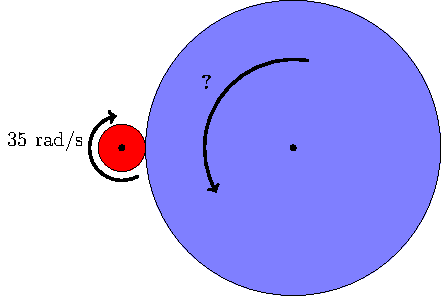
\includegraphics[width=7cm]{turntables.pdf}
    \caption{Original Figure.  A turntable is turned by a circular rubber roller in contact with it at their outer edges.  There is no slipping.}
    \label{turntables}
  \end{figure}

\mysubheading{Conceptual Questions}

\myquestion (CQ2) \label{1q-i}
Explain why centripetal acceleration changes the direction of velocity in circular motion but not its magnitude.

\myquestion (CQ3) In circular motion, a tangential acceleration can change the magnitude of the velocity but not its direction. Explain your answer.

\myquestion (Giancoli CQ1) 
A bicycle odometer (which counts revolutions and is calibrated to report distance traveled) is attached near the wheel axle and is calibrated for 27-inch wheels. What happens if you use it on a bicycle with 24-inch wheels?
\answer{it will always read too far}


\myquestion (Giancoli CQ2) Suppose a disk rotates at constant angular velocity.
(a) Does a point on the rim have radial and/or tangential acceleration?
(b) If the disk's angular velocity increases uniformly, does the point have radial and/or tangential acceleration?
(c) For which cases would the magnitude of either component of linear acceleration change?
\answer{(a) radial only; (b) both; (c) radial changes if there's an $\alpha$, tangential only changes if $\alpha$ changes.}

\myquestion (Giancoli MC1, modified) \label{1q-f}
Bonnie sits on the outer rim of a merry-go-round, and Jill sits midway between the center and the rim. The merry-go-round makes one complete revolution every 2~seconds. Who (if either) has the larger $v$ and who (if either) has the larger $\omega$?
\answer{Bonnie has larger $v$; they have the same $\omega$}



\myheading{Rotational Kinematic Equations}
\mysubheading{Problems}

% \myquestion (P5) 
% With the aid of a string, a gyroscope is accelerated from rest to 32~rad/s in 0.40~s.  (a) What is its angular acceleration?  (b) How many revolutions does it go through in the process?
% \answer{(a) \SI{80}{rad/s^2}; (b) 1.0 rev}

\myquestion (P8) \label{2p-i}
During a very quick stop, a car decelerates at \SI{7.00}{m/s^2}.
(a) What is the angular acceleration of its 0.280-m-radius tires, assuming they do not slip on the pavement?
(b) How many revolutions do the tires make before coming to rest, given their initial angular velocity is 95.0~rad/s ?
(c) How long does the car take to stop completely?
(d) What distance does the car travel in this time?
(e) What was the car's initial velocity?
(f) Do the values obtained seem reasonable, considering that this stop happens very quickly?
\answer{(a) \SI{-25.0}{rad/s^2};
        (b) 28.7 rev;
        (c) 3.80 s;
        (d) 50.7 m;
        (e) 26.6 m/s}


\myquestion (P6)
Suppose a piece of dust finds itself on a CD. If the spin rate of the CD is 500~rpm, and the piece of dust is 4.3~cm from the center, what is the total distance traveled by the dust in 3 minutes? (Ignore accelerations due to getting the CD rotating.)
\answer{405 m}


\myquestion (P7) 
A gyroscope slows from an initial rate of 32.0~rad/s at a rate of \SI{0.700}{rad/s^2}. (a) How long does it take to come to rest?
(b) How many revolutions does it make before stopping?
\answer{(a) 45.7~s; (b) 116~rev}





% \myquestion (P9) \textit{Everyday application:} 
% Suppose a yo-yo has a center shaft that has a 0.250 cm radius and that its string is being pulled.
% (a) If the string is stationary and the yo-yo accelerates away from it at a rate of \SI{1.50}{m/s^2}, what is the angular acceleration of the yo-yo?
% (b) What is the angular velocity after 0.750~s if it starts from rest?
% (c) The outside radius of the yo-yo is 3.50~cm. What is the tangential acceleration of a point on its edge?

%   \begin{figure}[H]
%     \centering
%     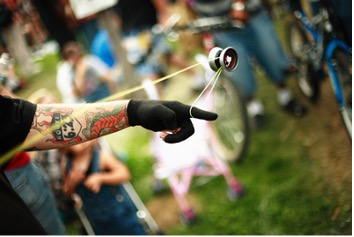
\includegraphics[width=6cm]{OS_10-35.jpg}
%     \caption{OpenStax Figure  10.35.  Yo-yos are amusing toys that display significant physics and are engineered to enhance performance based on physical laws. (credit: Beyond Neon, Flickr)}
%     \label{OS10.35}
%   \end{figure}


% \myquestion (Giancoli P17)
% An automobile engine slows down from 3500~rpm to 1200~rpm in 2.5~s.  Calculate (a) its angular acceleration, and (b) the total number of revolutions the engine makes in this time.

% \myquestion (Giancoli P18)
% A centrifuge accelerates uniformly from rest to 15,000~rpm in 240~s. Through how many revolutions did it turn in this time? 

% \myquestion (Giancoli P21)
% A wheel 31~cm in diameter accelerates uniformly from 240~rpm to 360~rpm in 6.8~s. How far will a point on the edge of the wheel have traveled in this time?

\myquestion (Giancoli P23) \label{2p-f}
A small rubber wheel is used to drive a large pottery wheel (similar to Figure~\ref{turntables} earlier). The two wheels are mounted so that their circular edges touch. The small wheel has a radius of 2.0~cm and accelerates at the rate of 7.2~rad/s$^2$, and it is in contact with the pottery wheel (radius 27.0~cm) without slipping. Calculate (a) the angular acceleration of the pottery wheel, and (b) the time it takes the pottery wheel to reach its required speed of 65~rpm. 
\answer{\SI{0.533}{\radian\per\second^2}; 12.77 s}



% \mysubheading{Conceptual Questions}

% \myquestion


\myheading{Torque}
\mysubheading{Problems}

\myquestion (Giancoli P24) \label{3p-i}
A 52-kg person riding a bike puts all her weight on each pedal when climbing a hill. The pedals rotate in a circle of radius 17~cm. (a) What is the maximum torque she exerts? (b) How could she exert more torque? 
\answer{\SI{86.63}{\meter\newton}}

 
 
% \myquestion (Giancoli P25)
% Calculate the net torque about the axle of the wheel shown in Figure~\ref{8-42}. Assume that a friction torque of \SI{0.60}{\meter\newton} opposes the motion.

% \GFig{42}{5cm}
 
\myquestion (Giancoli P26) \label{3p-f}
A person exerts a horizontal force of 42~N on the end of a door 96~cm wide. What is the magnitude of the torque if the force is exerted (a) perpendicular to the door and (b) at a $60^\circ$ angle to the face of the door? 
\answer{\SI{40.32}{\meter\newton}; \SI{34.92}{\meter\newton}}


\myquestion \textbf{Bonus} (Giancoli P28) \label{b1}
The bolts on the cylinder head of an engine require tightening to a torque of \SI{95}{m.N}. If a wrench is 28~cm long, what force perpendicular to the wrench must the mechanic exert at its end? If the six-sided bolt head is 15 mm across (Figure~\ref{8-44}), estimate the force applied near each of the six points by a wrench. 
\answer{340 N; 1800 N}


\GFig{44}{6cm}


\mysubheading{Conceptual Questions}

% \myquestion (Giancoli CQ3) 
% Can a small force ever exert a greater torque than a larger force? Explain.

\myquestion (Giancoli MC4) \label{3q-i}
The solid dot shown in Figure~\ref{8-36} is a pivot point. The board can rotate about the pivot. Which force shown exerts the largest magnitude torque on the board?
\answer{(c)}

\GFig{36}{6.5cm}

\myquestion (CQ7) \label{3q-f}
Give an example in which a small force exerts a large torque. Give another example in which a large force exerts a small torque.






\myheading{Rotational Dynamics}
\mysubheading{Problems}

\myquestion (Giancolli P30) \label{4p-i}
Determine the moment of inertia of a 10.8-kg sphere of radius 0.648~m when the axis of rotation is through its center.
\answer{\SI{1.81}{kg.m^2}}


\myquestion (Giancolli P32)
Estimate the moment of inertia of a bicycle wheel 67~cm in diameter. The rim and tire have a combined mass of 1.1~kg. The mass of the hub (at the center) can be ignored (why?).
\answer{\SI{0.123}{kg.m^2}}


% \myquestion (P11) 
% Calculate the moment of inertia of a skater given the following information. (a) The 60.0-kg skater is approximated as a cylinder that has a 0.110-m radius. (b) The skater with arms extended is approximately a cylinder that is 52.5 kg, has a 0.110-m radius, and has two 0.900-m-long arms which are 3.75 kg each and extend straight out from the cylinder like rods rotated about their ends.

\myquestion (P12) 
The triceps muscle in the back of the upper arm extends the forearm. This muscle in a professional boxer exerts a force of \SI{2.0e3}{N} with an effective perpendicular lever arm of 3.00~cm, producing an angular acceleration of the forearm of \SI{120}{rad/s^2}. What is the moment of inertia of the boxer's forearm?
\answer{\SI{0.500}{kg.m^2}}


% \myquestion (P13) 
% A soccer player extends her lower leg in a kicking motion by exerting a force with the muscle above the knee in the front of her leg. She produces an angular acceleration of \SI{30.0}{rad/s^2} and her lower leg has a moment of inertia of \SI{0.750}{kg.m^2}. What is the force exerted by the muscle if its effective perpendicular lever arm is 1.90~cm?

\myquestion (P14) 
Suppose you exert a force of 180 N tangential to a 0.280-m-radius 75.0-kg grindstone (a solid disk).(a) What torque is exerted? (b) What is the angular acceleration assuming negligible opposing friction? (c) What is the angular acceleration if there is an opposing frictional force of 20.0~N exerted 1.50~cm from the axis?
\answer{(a) \SI{50.4}{m.N}; (b) \SI{17.1}{rad/s^2}; (c) \SI{17.0}{rad/s^2}}


% \myquestion (Giancoli P40)
% A potter is shaping a bowl on a potter's wheel rotating at constant angular velocity of 5.03~rad/s (Figure~\ref{8-48}). The friction force between her hands and the clay is 1.5~N total. (a) How large is her torque on the wheel, if the diameter of the bowl is 9.0~cm? (b) How long would it take for the potter's wheel to stop if the only torque acting on it is due to the potter's hands? The moment of inertia of the wheel and the bowl is \SI{0.11}{kg.m^2}. 

% \GFig{48}{5cm}

 
\myquestion (Giancoli P41)
A dad pushes tangentially on a small hand-driven merry-go-round and is able to accelerate it from rest to a frequency of 15~rpm in 10.0~s. Assume the merry-go-round is a uniform disk of radius 2.5~m and has a mass of 560~kg, and two children (each with a mass of 25~kg) sit opposite each other on the edge. Calculate the torque required to produce the acceleration, neglecting frictional torque. What force is required at the edge? (\emph{Hint:} Treat each child as a particle and calculate the moment of inertia of the merry-go-round plus the two children.)
\answer{\SI{324}{\meter\newton}; \SI{129.6}{\newton}}

 
\myquestion (Giancoli P45)
To get a flat, uniform cylindrical satellite spinning at the correct rate, engineers fire four tangential rockets as shown in figure~\ref{8-50}. Suppose that the satellite has a mass of 3600~kg and a radius of $R=4.0$~m, and that the rockets each add a mass of 250 kg and can be treated as particles. What is the steady force required of each rocket if the satellite is to reach 32~rpm in 5.0~min, starting from rest?
\answer{31.3 N}


\GFig{50}{4.2cm}


\myquestion (Giancoli P44) \label{4p-f}
A centrifuge rotor rotating at 9200~rpm is shut off and is eventually brought uniformly to rest by a frictional torque of \SI{1.20}{m.N}. If the mass of the rotor is 3.10~kg and it can be approximated as a solid cylinder of radius 0.0710~m, through how many revolutions will the rotor turn before coming to rest, and how long will it take? 
\answer{480 rev; 6.3 s}


\myquestion \textbf{Bonus} (Giancoli P36) \label{b2}
Assume that a 1.00-kg ball is thrown solely by the action of the forearm, which rotates about the elbow joint under the action of the triceps muscle, Figure~\ref{8-46}. The ball is accelerated uniformly from rest to 8.5~m/s in 0.38~s, at which point it is released. Calculate (a) the angular acceleration of the arm, and (b) the force required of the triceps muscle. Assume that the forearm has a mass of 3.7~kg and rotates like a uniform rod about an axis at its end. 
\answer{(a) \SI{72}{rad/s^2}; (b) 620 N}


\GFig{46}{4cm}


\mysubheading{Conceptual Questions}

\myquestion (CQ8) \label{4q-i}
While reducing the mass of a racing bike, the greatest benefit is realized from reducing the mass of the tires and wheel rims. Why does this allow a racer to achieve greater accelerations than would an identical reduction in the mass of the bicycle's frame?
%
  \begin{figure}[H]
    \centering
    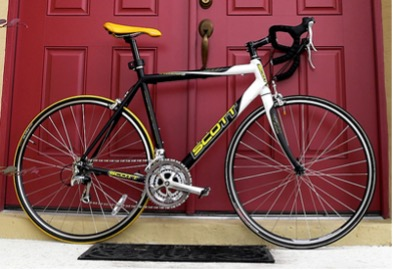
\includegraphics[width=5.5cm]{OS_10-30.jpg}
    \caption{OpenStax Fig. 10.30.  The image shows a side view of a racing bicycle. Can you see evidence in the design of the wheels on this racing bicycle that their moment of inertia has been purposely reduced? (credit: Jesús Rodriguez)}
  \end{figure}

\myquestion (Giancoli CQ9)
The moment of inertia of a rotating solid disk about an axis through its center of mass is $\frac{1}{2}MR^2$. Suppose instead that a parallel axis of rotation passes through a point on the edge of the disk. Will the moment of inertia be the same, larger, or smaller? Explain why.
\answer{larger}

\myquestion (CQ6) 
Why is the moment of inertia of a hoop that has a mass $M$ and a radius $R$ greater than the moment of inertia of a disk that has the same mass and radius? Why is the moment of inertia of a spherical shell that has a mass $M$ and a radius $R$ greater than that of a solid sphere that has the same mass and radius?


\myquestion (Giancoli MC6) \label{4q-f}
Two spheres have the same radius and equal mass. One sphere is solid, and the other is hollow and made of a denser material. Which one has the bigger moment of inertia about an axis through its center?
\answer{the hollow sphere has a larger $I$}



\myheading{Rotational KE}
\mysubheading{Problems}

\myquestion (P23a) \label{5p-i}
Calculate the rotational kinetic energy of Earth on its axis. The mass of the earth is \SI{5.98e24}{kg} and its radius is \SI{6.38e6}{m}.
\answer{\SI{2.57e29}{J}}



\myquestion (Giancoli P50) 
A centrifuge rotor has a moment of inertia of \SI{3.25e-2}{kg.m^2}. How much energy is required to bring it from rest to 8750~rpm?
\answer{13,640 J}


\myquestion (Giancoli P52)
A bowling ball of mass 7.25~kg and radius 10.8~cm rolls without slipping down a lane at 3.10~m/s. Calculate its total kinetic energy.
\answer{48.8 J}


\myquestion (P22) \label{5p-f}
What is the final velocity of a hoop that rolls without slipping down a 5.00-m-high hill, starting from rest?
\answer{7.00 m/s}


% \myquestion (Giancoli P56)
% A sphere of radius $r=34.5$~cm and mass $m=1.80$~kg starts from rest and rolls without slipping down a $30^\circ$ incline that is 10.0~m long. (a) Calculate its translational and rotational speeds when it reaches the bottom. (b) What is the ratio of translational to rotational kinetic energy at the bottom? Avoid putting in numbers until the end so you can answer: (c) do your answers in (a) and (b) depend on the radius of the sphere or its mass?

\mysubheading{Conceptual Questions}

\myquestion (Giancoli MC7) \label{5q-i}
Two wheels having the same radius and mass rotate at the same angular velocity (Figure~\ref{8-38}). One wheel is made with spokes so nearly all the mass is at the rim. The other is a solid disk. Which one has the larger rotational KE?
\answer{the one with spokes has more $KE_r$}


\GFig{38}{6cm}


\myquestion (Giancoli CQ12) \label{5q-f}
A sphere and a cylinder have the same radius and the same mass. They start from rest at the top of an incline.
(a) Which reaches the bottom first?
(b) Which has the greater speed at the bottom?
(c) Which has the greater total kinetic energy at the bottom?
(d) Which has the greater rotational kinetic energy?
\answer{(a) sphere; (b) sphere; (c) equal; (d) cylinder}

% \myquestion (Giancoli MC8) If you used 1000~J of energy to throw a ball, would it travel faster if you threw the ball so that it was also rotating or so that it wasn't rotating?  (Ignore Air Resistance)




% \myquestion (CQ9) A ball slides up a frictionless ramp. It is then rolled without slipping and with the same initial velocity up another frictionless ramp (with the same slope angle). In which case does it reach a greater height, and why?


\myheading{Angular Momentum}
\mysubheading{Problems}

\myquestion (P39) \label{6p-i}
A playground merry-go-round has a mass of 120~kg and a radius of 1.80~m and it is rotating with an angular velocity of 0.500~rev/s. What is its angular velocity after a 22.0-kg child gets onto it by grabbing its outer edge? The child is initially at rest.  The merry-go-round is a solid disk and the child can be modeled as a particle.
\answer{2.30 rad/s}


\myquestion (P40) Three children are riding on the edge of a merry-go-round that is 100~kg, has a 1.60-m radius, and is spinning at 20.0~rpm. The children have masses of 22.0, 28.0, and 33.0~kg. If the child who has a mass of 28.0~kg moves to the center of the merry-go-round, what is the new angular velocity in rpm?
\answer{25.3 rpm}





% \myquestion (Giancoli P64)
% A diver (such as the one shown in Figure~\ref{8-28}) can reduce her moment of inertia by a factor of about 3.5 when changing from the straight position to the tuck position. If she makes 2.0~rotations in 1.5~s when in the tuck position, what is her angular speed (rev/s) when in the straight position?

% \GFig{28}{5cm}


\myquestion (Giancoli P65) \label{6p-f}
A figure skater can increase her spin rotation rate from an initial state of 1.0~rev every 1.5~s to a final rate of 2.5~rev/s.  If her initial moment of inertia is \SI{4.6}{kg.m^2}, what is her final moment of inertia?  How does she physically accomplish this change?
\answer{\SI{1.23}{\kilo\gram.\meter^2}}


\myquestion \textbf{Bonus} (Giancoli P67) \label{b3}
A person of mass 75~kg stands at the center of a rotating merry-go-round platform of radius 3.0~m and moment of inertia \SI{820}{kg.m^2}. The platform rotates without friction with angular velocity 0.95~rad/s. The person walks radially to the edge of the platform. (a) Calculate the angular velocity when the person reaches the edge. (b) Calculate the rotational kinetic energy of the system of platform plus person before and after the person's walk.
\answer{(a) 0.52 rad/s; (b) 370 J, 200 J}


% \myquestion \textbf{Bonus} (Giancoli P72)
% A uniform disk turns at 3.3~rev/s around a frictionless central axis. A nonrotating rod, of the same mass as the disk and length equal to the disk's diameter, is dropped onto the freely spinning disk, Figure~\ref{8-56}. They then turn together around the axis with their centers superposed. What is the angular frequency in rev/s of the combination?

% \GFig{56}{3cm}



\vspace*{\stretch{1}}
\columnbreak

\mysubheading{Conceptual Questions}


% \myquestion (Giancoli P62a)
% A person stands, hands at his side, on a platform that is rotating at a rate of 0.90~rev/s. If he raises his arms to a horizontal position, Figure~\ref{8-55}, the speed of rotation decreases to 0.60~rev/s. Why? 

% \GFig{55}{4cm}


% \myquestion (CQ18) Describe how work is done by a skater pulling in her arms during a spin. In particular, identify the force she exerts on each arm to pull it in and the distance each moves, noting that a component of the force is in the direction moved. Why is angular momentum not increased by this action?

\myquestion (CQ23) \label{6q-i}
Competitive divers pull their limbs in and curl up their bodies when they do flips. Just before entering the water, they fully extend their limbs to enter straight down. Explain the effect of both actions on their angular velocities. Also explain the effect on their angular momenta.

  \begin{figure}[H]
    \centering
    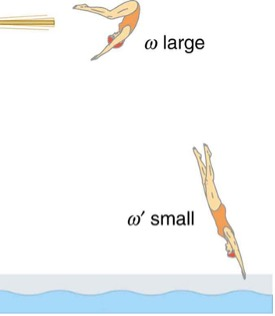
\includegraphics[width=4.5cm]{OS_10-33.jpg}
    \caption{OpenStax Figure 10.33.  The diver spins rapidly when curled up and slows when she extends her limbs before entering the water.}
    \label{OS10.33}
  \end{figure}

\myquestion (Giancoli MC13) 
Suppose you are sitting on a rotating stool holding a 2-kg mass in each outstretched hand. If you suddenly drop the masses, what will happen to your angular velocity?
\answer{speed up}


\myquestion (CQ14)  \label{6q-f}
Suppose a child walks from the outer edge of a rotating merry-go round to the inside. Does the angular velocity of the merry-go-round increase, decrease, or remain the same? Explain your answer.
\answer{speed up}

% \vspace*{\stretch{1}}
% \columnbreak
   
% \myquestion (CQ15)
% Suppose a child gets off a rotating merry-go-round. Does the angular velocity of the merry-go-round increase, decrease, or remain the same if: (a) He jumps off radially? (b) He jumps backward to land motionless? (c) He jumps straight up and hangs onto an overhead tree branch? (d) He jumps off forward, tangential to the edge? Explain your answers. (Refer to Figure~\ref{OS10.32}).
% \answer{(a) speed up; (b) speed up; (c) speed up; (d) unable to say}


%   \begin{figure}[H]
%     \centering
%     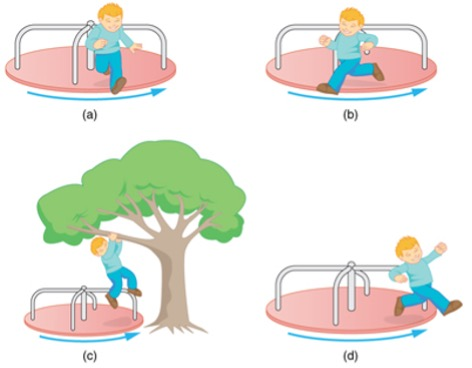
\includegraphics[width=6cm]{OS_10-32.jpg}
%     \caption{OpenStax Figure 10.32.  A child may jump off a merry-go-round in a variety of directions.}
%     \label{OS10.32}
%   \end{figure}

% \myquestion (Giancoli MC10) A small mass $m$ on a string is rotating without friction in a circle. The string is shortened by pulling it through the axis of rotation without any external torque, Figure~\ref{8-39}. What happens to the angular velocity of the object?

% \GFig{39}{5cm}








% \myquestion (CQ1) Analogies exist between rotational and translational physical quantities. Identify the rotational term analogous to each of the following: acceleration, force, mass, translational kinetic energy, linear momentum.

\end{myquestions}

\end{document}